\chapter{Matrices de confusión y trazabilidad de los resultados}
\label{anexo:confusiones}
Las Figuras~\ref{fig:cm-svm-32} a~\ref{fig:cm-net5-64} presentan las seis matrices de confusión completas. Las etiquetas corresponden a las categorías oficiales; cada fila se normalizó por su soporte y cada celda expresa la proporción de predicciones para una categoría real. Los conteos enteros pueden recuperarse de los archivos de predicciones por objeto conservados en el repositorio.

\begin{figure}[p]\centering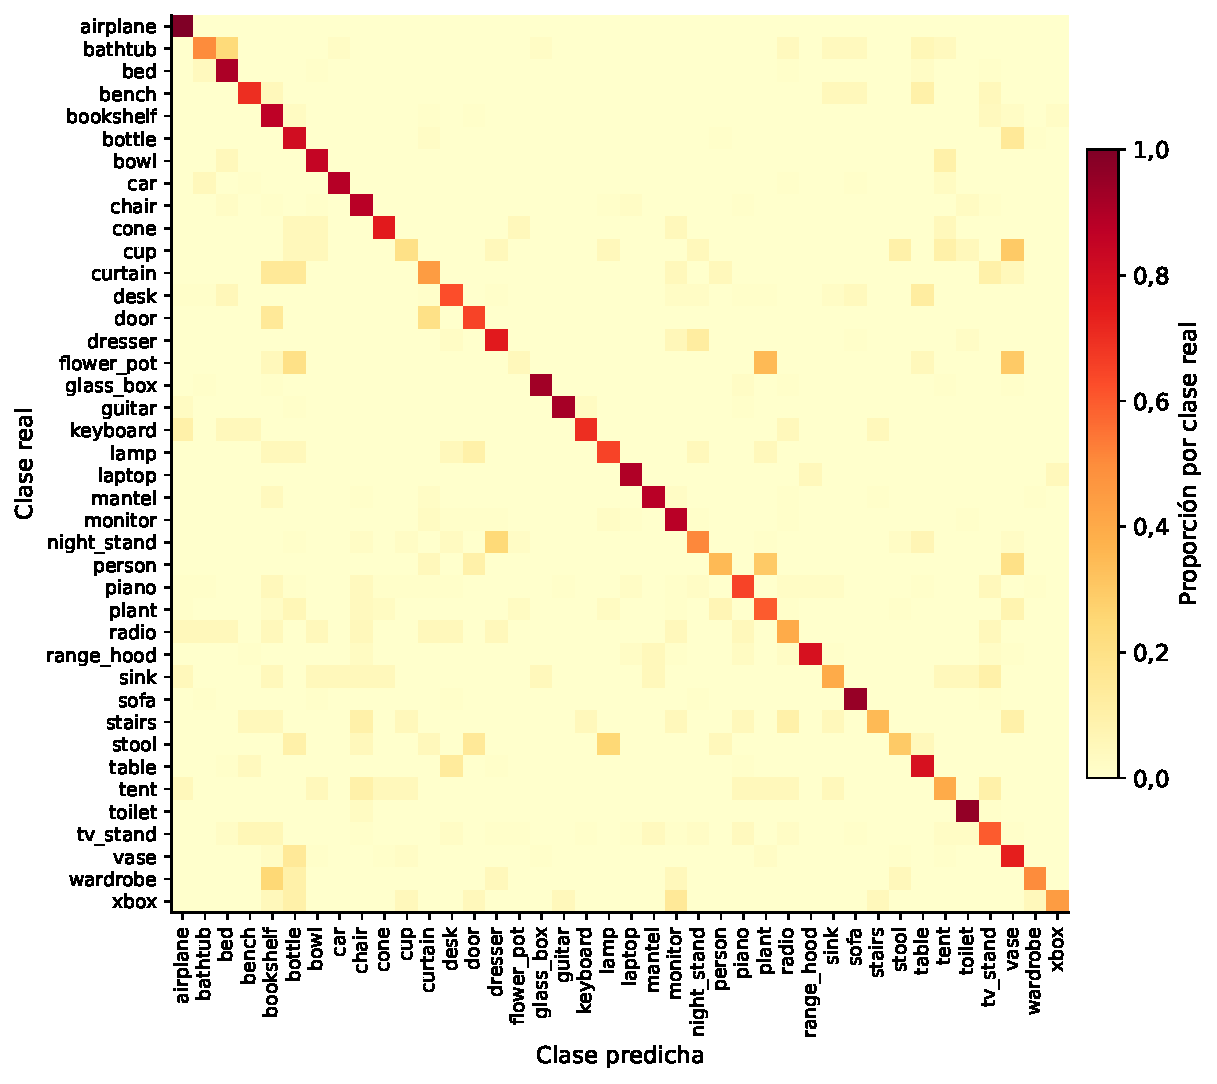
\includegraphics[width=\textwidth]{Figuras/cierre_cm_svm_32.pdf}
\caption{Matriz de confusión de SVM en $32^3$, normalizada por fila sobre los 2\,468 objetos de prueba. Elaboración propia a partir de las predicciones versionadas.}\label{fig:cm-svm-32}\end{figure}

\begin{figure}[p]\centering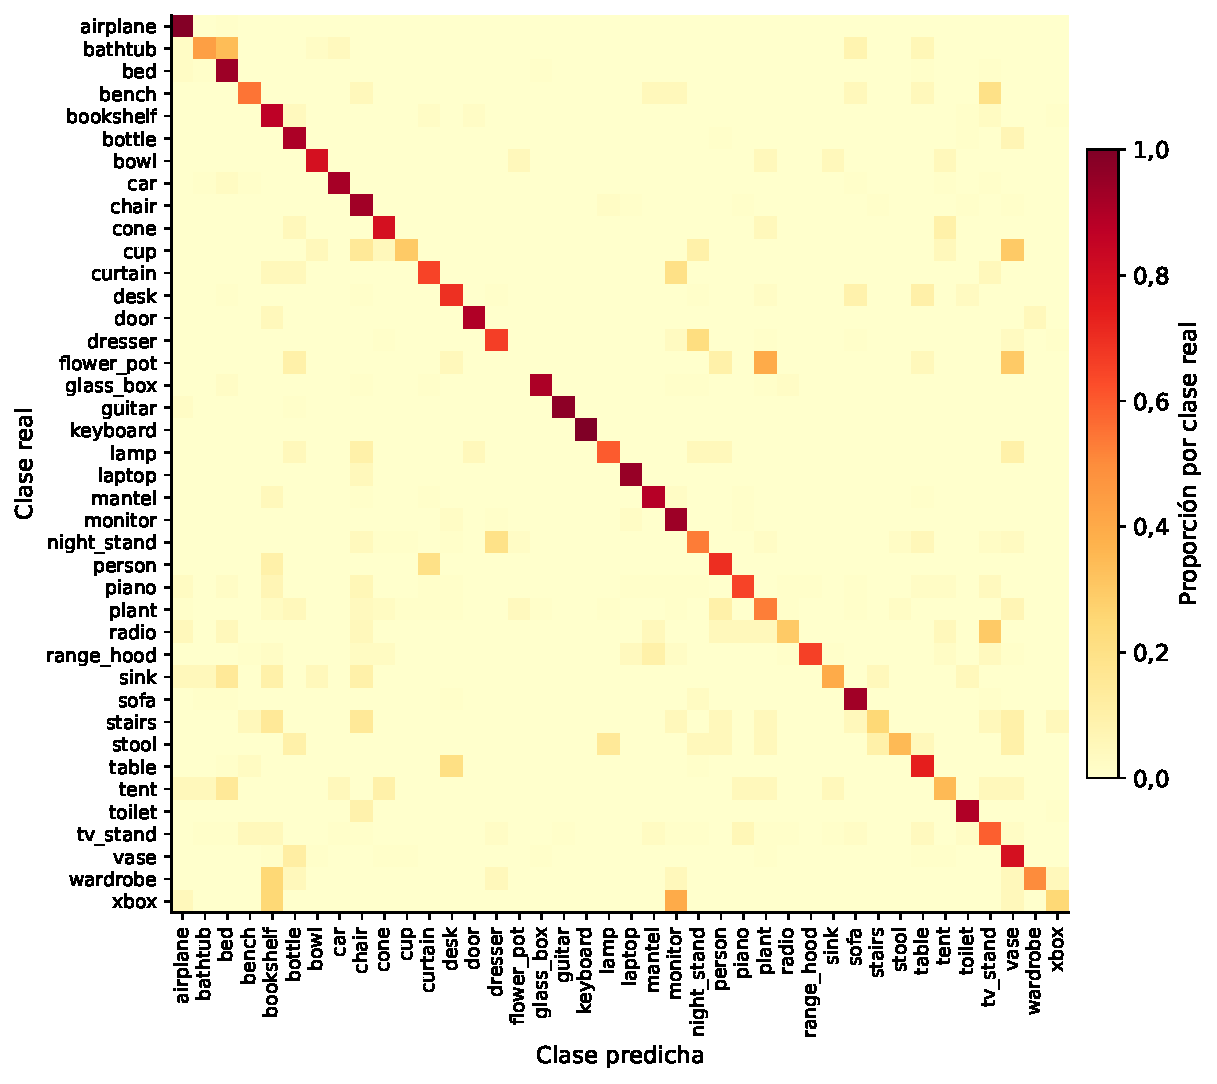
\includegraphics[width=\textwidth]{Figuras/cierre_cm_rf_32.pdf}
\caption{Matriz de confusión del Bosque Aleatorio en $32^3$, normalizada por fila sobre los 2\,468 objetos de prueba. Elaboración propia a partir de las predicciones versionadas.}\label{fig:cm-rf-32}\end{figure}

\begin{figure}[p]\centering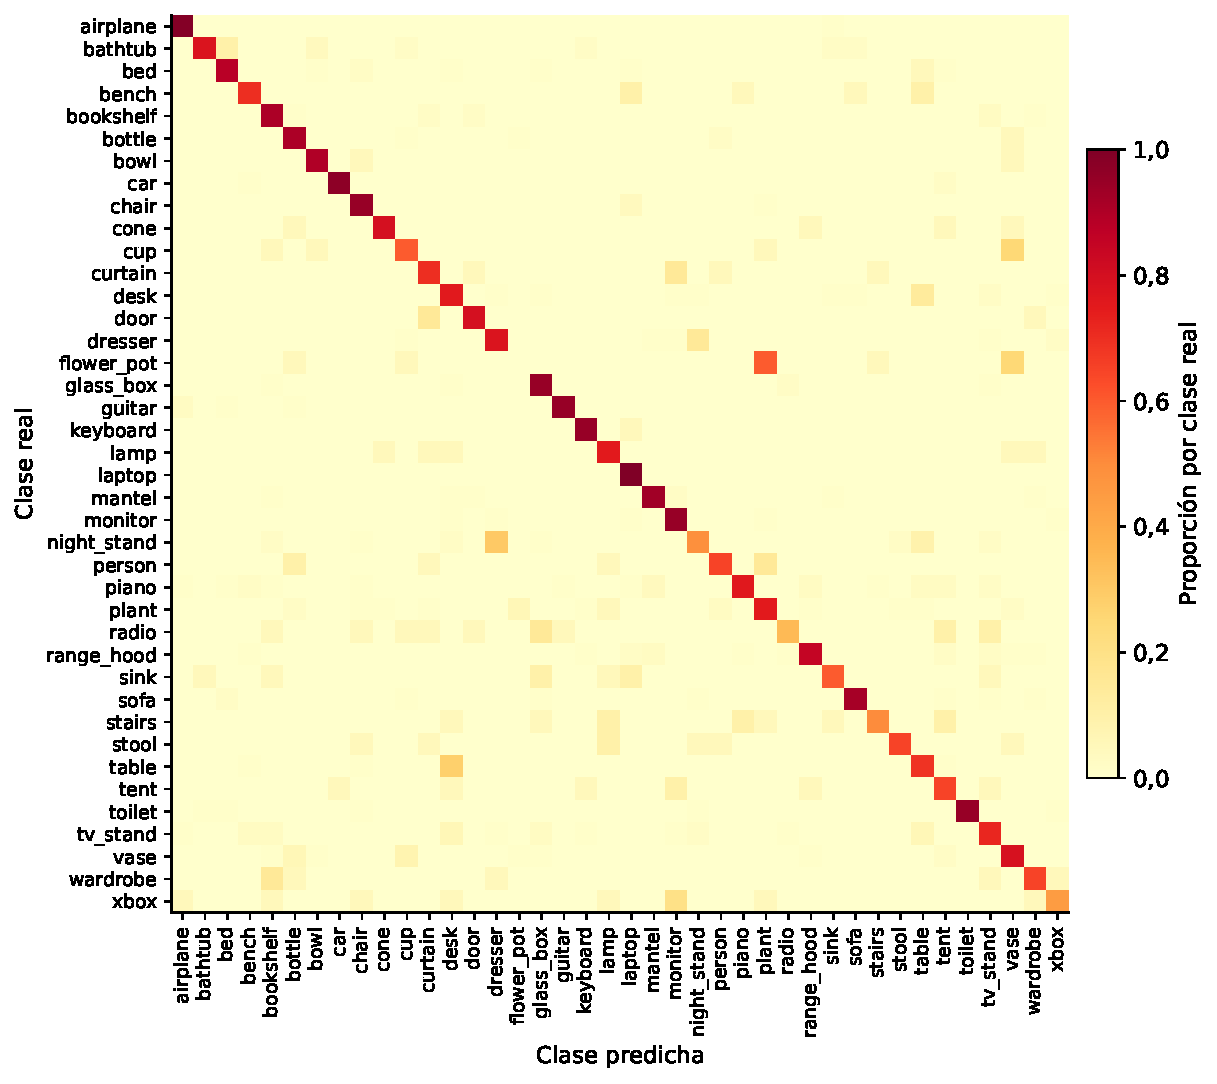
\includegraphics[width=\textwidth]{Figuras/cierre_cm_net5_32.pdf}
\caption{Matriz de confusión de Net5 en $32^3$, normalizada por fila sobre los 2\,468 objetos de prueba. Elaboración propia a partir de las predicciones versionadas.}\label{fig:cm-net5-32}\end{figure}

\begin{figure}[p]\centering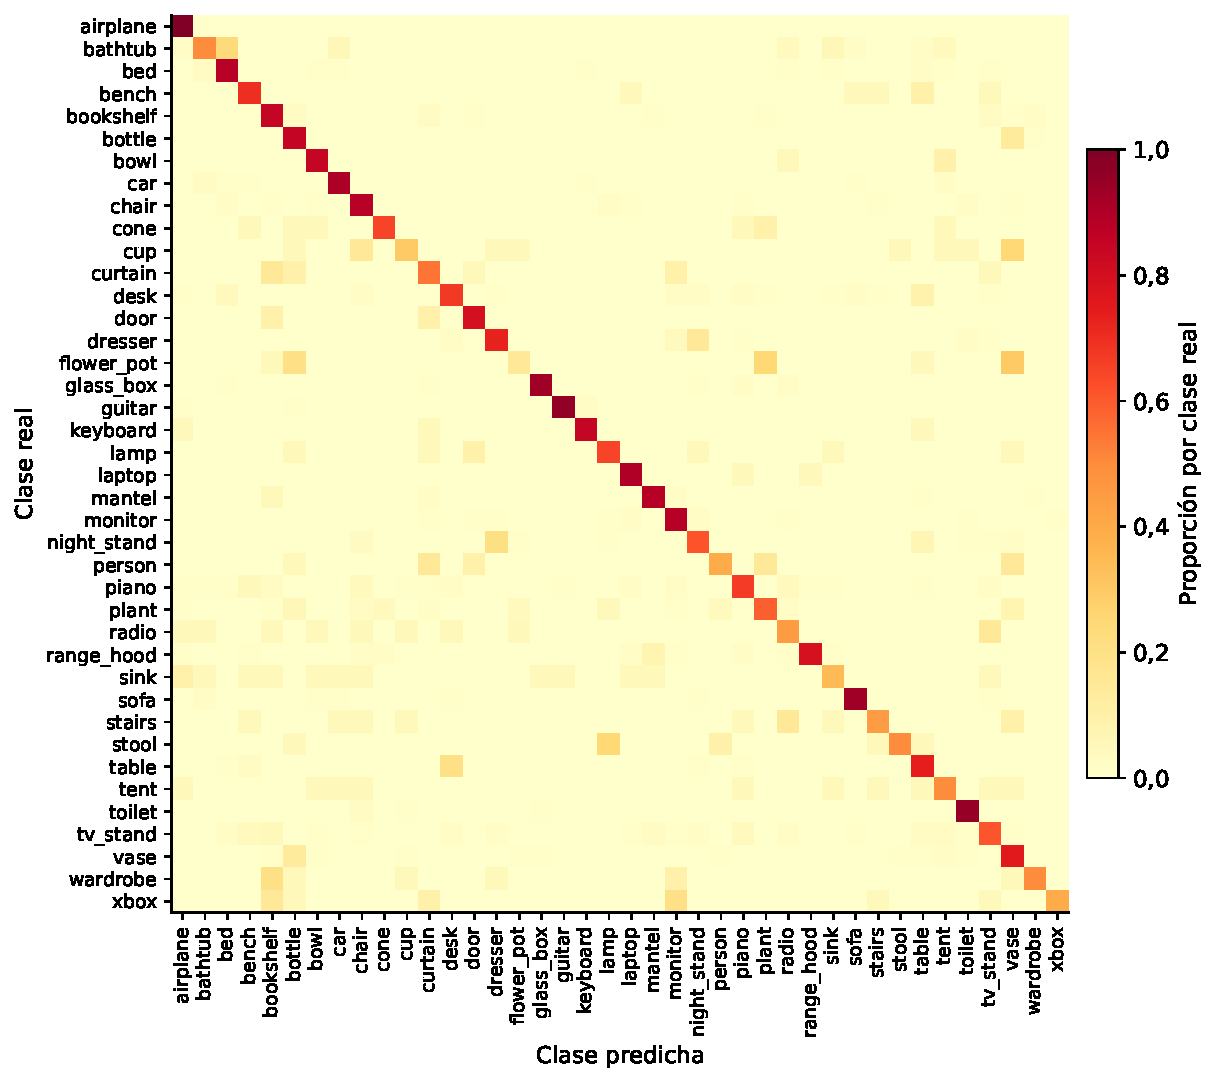
\includegraphics[width=\textwidth]{Figuras/cierre_cm_svm_64.pdf}
\caption{Matriz de confusión de SVM en $64^3$, normalizada por fila sobre los 2\,468 objetos de prueba. Elaboración propia a partir de las predicciones versionadas.}\label{fig:cm-svm-64}\end{figure}

\begin{figure}[p]\centering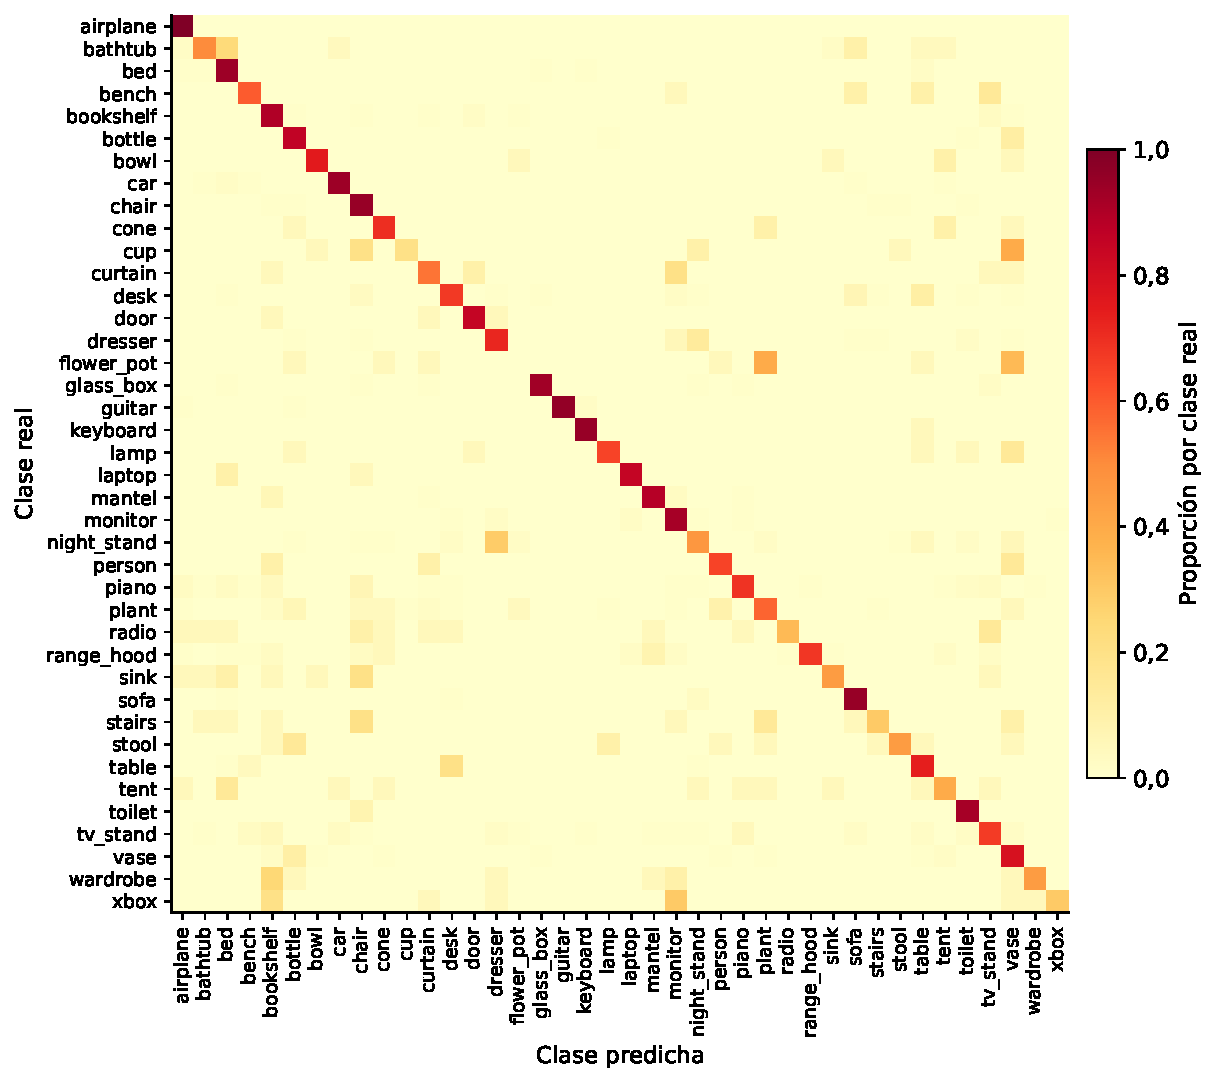
\includegraphics[width=\textwidth]{Figuras/cierre_cm_rf_64.pdf}
\caption{Matriz de confusión del Bosque Aleatorio en $64^3$, normalizada por fila sobre los 2\,468 objetos de prueba. Elaboración propia a partir de las predicciones versionadas.}\label{fig:cm-rf-64}\end{figure}

\begin{figure}[p]\centering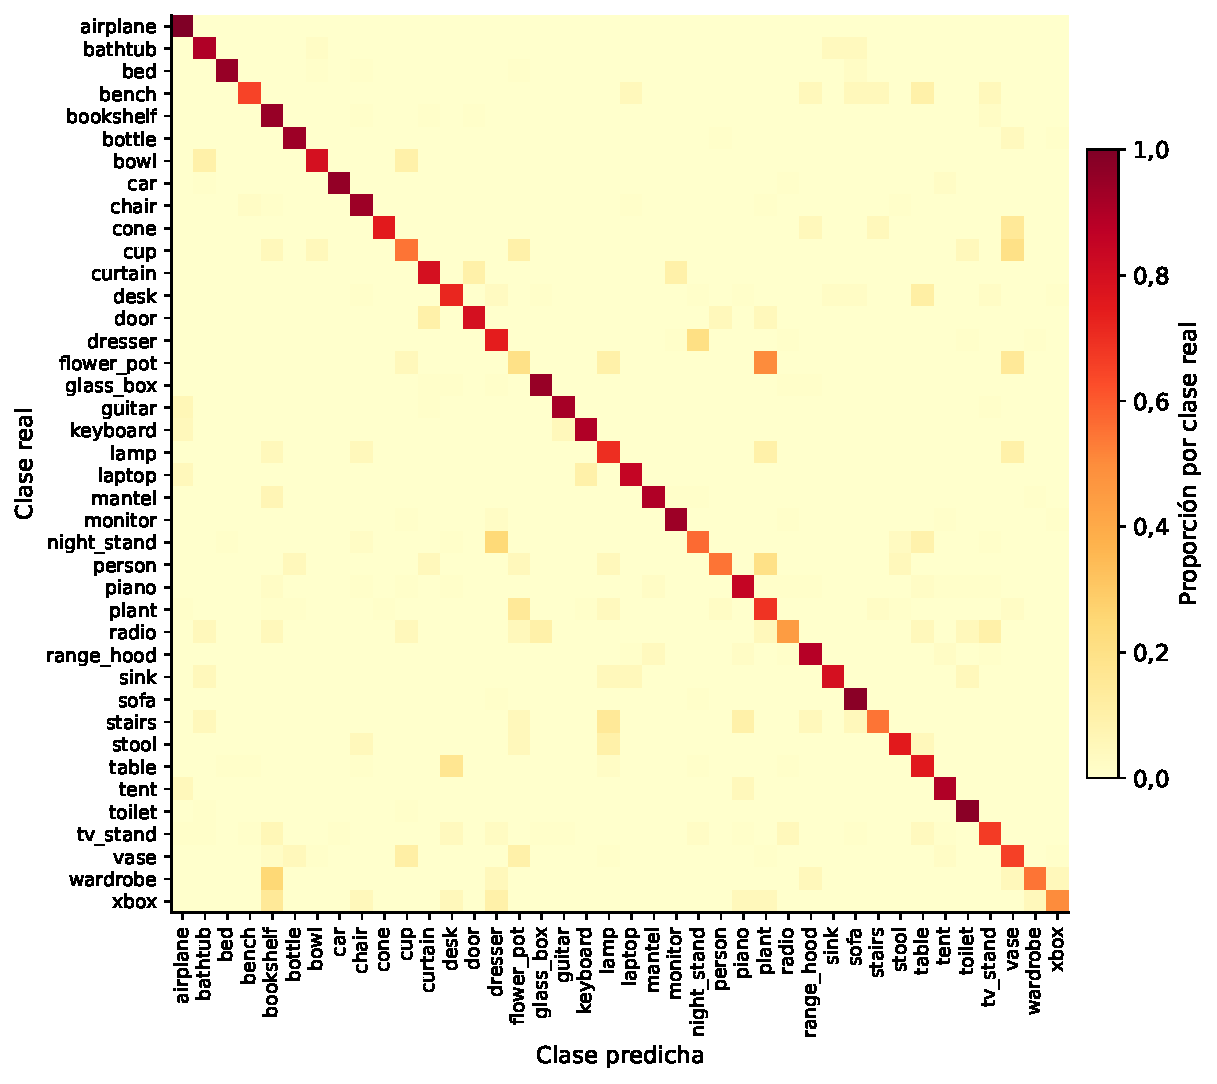
\includegraphics[width=\textwidth]{Figuras/cierre_cm_net5_64.pdf}
\caption{Matriz de confusión de Net5 en $64^3$, normalizada por fila sobre los 2\,468 objetos de prueba. Elaboración propia a partir de las predicciones versionadas.}\label{fig:cm-net5-64}\end{figure}

\clearpage
\section{Localización de la evidencia}
El repositorio del proyecto~\parencite{lopez2026octree} se encuentra en \url{https://github.com/ricardoal94/Octree}. La versión consolidada consultada fue el commit \href{https://github.com/ricardoal94/Octree/tree/64b8835dd94a409122bd0b01bcfc5a501e351095}{\texttt{64b8835}}; el enlace conduce al identificador completo. Los datos de la comparación principal están en \path{resultados/Objetivos_4_y_5_comparacion}; la reevaluación está en \path{resultados/Objetivos_4_y_5_reevaluacion_2026-09-27}. Los archivos \path{analisis.json}, \path{tiempos.json} y \path{memoria.json} contienen las métricas agregadas. Los archivos \path{predicciones_R32.csv} y \path{predicciones_R64.csv} permiten reconstruir conteos, matrices y contrastes.

La validación geométrica se documentó en \path{validacion_chair_0001.json}, en \path{resultados/objetivo1} y en \path{resultados/objetivo1/muestra_controlada}. Los resúmenes de entrenamiento y sus historiales se conservaron en el subdirectorio \path{resultados/oficiales} de la comparación. Las instrucciones del repositorio describen la ubicación de los modelos y datos necesarios para repetir las etapas. El paquete documental incluye una copia de la evidencia numérica utilizada para construir sus tablas y figuras; no reemplaza la distribución de los modelos y del conjunto de datos.
